\documentclass[letterpaper,12pt,oneside]{report}

\usepackage[T1]{fontenc}
\usepackage[utf8]{inputenc}
\usepackage[UKenglish]{babel}
\usepackage{graphicx}
\usepackage{tikz}
\usepackage{listings}
\usepackage{color}

\definecolor{dkgreen}{rgb}{0,0.6,0}
\definecolor{gray}{rgb}{0.5,0.5,0.5}
\definecolor{mauve}{rgb}{0.58,0,0.82}

\lstset{frame=tb,
  language=Java,
  aboveskip=3mm,
  belowskip=3mm,
  showstringspaces=false,
  columns=flexible,
  basicstyle={\small\ttfamily},
  numbers=none,
  numberstyle=\tiny\color{gray},
  keywordstyle=\color{blue},
  commentstyle=\color{dkgreen},
  stringstyle=\color{mauve},
  breaklines=true,
  breakatwhitespace=true,
  tabsize=3
}
\graphicspath{{./figs/}}
\usepackage{setspace}
\usepackage[top=1in, left=1.25in, right=1.25in, bottom=1in]{geometry}
\usepackage{graphics}
\usepackage{hyperref}
\hypersetup{
    colorlinks=true,
    linkcolor=blue,
    filecolor=magenta,      
    urlcolor=cyan,
}
\begin{document}
\begin{center}
\large{\textbf{
Veermata Jijabai Technological Institute,Mumbai\\
\\ 
        (Autonomous Institute Affiliated to University of Mumbai)\\
               2018 - 2019} \\
\vspace{15mm}
}
\Large{
Nikita Masand\\
Mentor: Prof. Pranav Nerurkar\\
SY IT\\
171081054\\
\vspace{15mm}
}
\par
\Huge{
\textbf{Game Theory}\\
}
\vspace{8mm}

\includegraphics[]{logo.jpeg}
\par

\Large{
\vspace{25mm}
Department Of Computer Engineering And Information Technology\\
}
\end{center}
%\author{Nikita Masand}
%\title{Game Theory}
%\faculty{   Veermata Jijabai Technological Institute,Mumbai}
%\degree{}
%\supervisor{}
%\cityandyear{}
%\logouni{}
%\logofac{}
\begin{titlepage}
\vspace*{2\baselineskip}
\begin{center} \begin{Huge} \textbf{CERTIFICATE}\end{Huge} \end{center} 
\vspace*{2\baselineskip}
\Large
This  is  to  certify  that, \textbf{Nikita Masand (ID-171081054)} , a  student  of  \textbf{Bachelor  Of  Technology (Information Technology)} has  completed  the  lab  report  held  in  Jan-Feb  2019  for  thesis on Game Theory   to  our  satisfaction.
\vspace*{14\baselineskip}\\
Mr.Pranav Nerurkar \hspace{0.8in}    \hspace{0.5in}           Dr. V. B. Nikam\\
\hspace{0.8in} Supervisor  \hspace{1in}          \hspace{1.1in}  HOD of CE \& IT
\vspace*{2\baselineskip}
\\Date:\\Place:                   
\end{titlepage}

%------------------------------------------------------------------------
%-------------------------------------------------------------------------------

%Certificate part(Fourth Page)
\vspace*{3\baselineskip}
\begin{center}\begin{Huge}\textbf{Declaration of the Student}\end{Huge}\end{center}
\vspace*{2\baselineskip}
\begin{Large}
I declare that this written submission represents my ideas in my own words and where others' ideas or words have been included, I have adequately cited and referenced the original sources.\\

I also declare that I have adhered to all principles of academic honesty and integrity and have not misrepresented or fabricated or falsified any idea/data/fact/source in my submission.\\

I understand that any violation of the above will be cause for disciplinary action by the Institute and can also evoke penal action from the sources which have thus not been properly cited or from whom proper permission has not been taken when needed.
\end{Large}
\vspace*{8\baselineskip}
\\Nikita Masand \\
\hspace{0.5in}(Reg no : 171081054)   \hspace{2.5in} Date: \line(1,0){100}
\newpage
\begin{centering}
\Huge{
\textbf{Acknowledgements}\\
}
\vspace{5mm}
\end{centering}
\begin{Large}
My sincere thanks goes to Dr. Dhiren Patel, Director of Veermata Jijabai Technological Institute, Mumbai who provided me an opportunity to work as a research scholar and gave me access to the laboratory and research facilities which helped me to conduct this research.I would like to express my sincere gratitude to my supervisor Mr. Pranav Nerurkar for the patience, motivation, and immense knowledge whose guidance helped me in all the time of research and writing of this report.I thank our Head of the Department Dr.  V. B. Nikam, for extending his invaluable support.  I would also thank my institute and the department’s faculty members without whom this research work would have been a distant reality.I also extend my heartfelt thanks to my family and well wishers. Thank you for always encouraging
me and for bringing so much love and happiness to my life!

\end{Large}
\vspace*{8\baselineskip}
%---------------------------------------------------
\newpage
\begin{Large}
\begin{centering}
\textbf{PREFACE}
\\
\end{centering}
\vspace{5mm}
Game theory has found its applications in numerous fields such as Economics, Social Science, Political Science, Evolutionary Biology. Game theory is now finding its applications in computer science. The nature of computing is changing because of success of Internet and the revolution in Information technology. The advancement in technologies have made it possible to commodities the components such as network, computing, storage and software. In the new paradigm, there are multiple entities (hardware, software agents, protocols etc.) that work on behalf of different autonomous bodies (such as a user, a business etc.) and provide services to other similar entities. Internet has made is possible for many such geographically distributed antonymous entities to interact with each other and provide various services. These entities will work  for their respective owners to achieve their individual goals (maximize their individual payoffs), as opposed to obtaining a system optima (that is socially desirable). This results in an entirely different paradigm of computing where the "work" is performed in a completely distributed/decentralized fashion by different entities where the primary objective of each entity  is to maximize the objective of its owner. Therefore, it is important to study traditional computer science concepts such as algorithm design, protocols, performance optimization under a game-theoretic model.  


\end{Large}
%--------------------------------------------------------------------------------
\Large

\tableofcontents
\listoffigures
\listoftables
\newpage
\chapter{What is Game Theory?}
Game Theory can be regarded as a multi-agent decision problem. Which means there are many people contending for limited rewards/payoffs. They have to make certain moves on which their payoff depends. These people have to follow certain rules  while making these moves.  Each player is supposed to behave rationally.\\
\textbf{Rationality:} In the language of Game Theory rationality implies that each player tries to maximize his/her payoff irrespective to what other players are doing.
In essence each player has to decide a set of moves which are in accordance with the rules of the game and which maximize his/her rewards.\\
Game Theory can be classified in two branches
\begin{enumerate}
    \item Non co-operative game theory :  In this case the players work independently without assuming anything about what other players are doing.
    \item Co-operative game theory: Here players may co-operate with one another.
\end{enumerate}
Game Theory has found applications in Economic, Evolutionary Biology, Sociology, Political Science etc, now Its finding applcations in Computer Science. 


\newpage
\section{What is a Game?}
\begin{quote}
    Game: A competitive activity involving skill, chance, or endurance on the part of two or more persons who play according to a set of rules, usually for their own amusement or for that of spectators.\\
\end{quote}
\begin{figure}
    \centering
    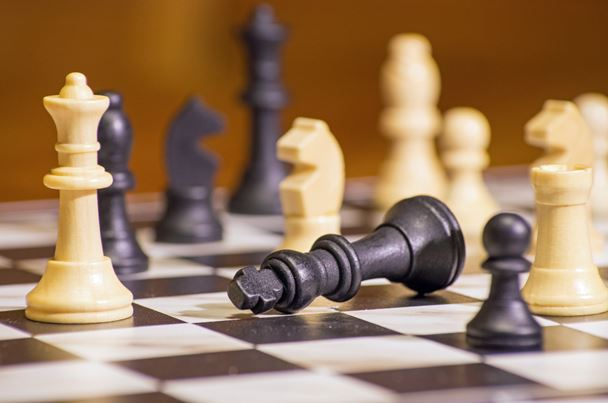
\includegraphics[]{game.jpg}
    \caption{gametheory}\\
    Source: https://cdn.static-economist.com/sites/default/
    \label{game:1}
\end{figure}
After learning how to play the game tick-tack-toe, you probably discovered a strategy of play that enables you to achieve at least a draw and even win if your opponent makes a mistake and you notice it. Sticking to that strategy ensures that you will not lose.

This simple game illustrates the essential aspects of what is now called game theory. In it, a game is the set of rules that describe it. An instance of the game from beginning to end is known as a play of the game. And a pure strategy--such as the one you found for tick-tack-toe--is an overall plan specifying moves to be taken in all eventualities that can arise in a play of the game. A game is said to have perfect information if, throughout its play, all the rules, possible choices, and past history of play by any player are known to all participants. Games like tick-tack-toe, backgammon and chess are games with perfect information and such games are solved by pure strategies. But whereas you may be able to describe all such pure strategies for tick-tack-toe, it is not possible to do so for chess, hence the latter's age-old intrigue.


A game has the following
\begin{table}[h!]
  \begin{center}
    \caption{Components}
    \label{tab:table1}
    \begin{tabular}{l|S|r}
      \hline
    Set of Players & $\mathrm { D } = \left\{\mathrm {P}_{\mathrm{i }}|1<=\mathrm{i}<=\mathrm{n}\right\}$\\
      Set of rules & R \\
      Set of Strategies & $\mathrm { S } _ { \mathrm {i} } \text { for each player } \mathrm { P } _ { \mathrm { i } }$ \\
      Set of Outcomes & O\\
      Pay off & u for each outcome
    \end{tabular}
  \end{center}
\end{table}

\newpage
\section{Examples of Game}
\subsection{Coin Matching Game}
Two players choose independently either Head or Tail and report it to a central authority. If both choose the same side of the coin , player 1 wins, otherwise 2 wins.

A game has the following :-
\begin{enumerate}
    \item \textbf{Set of Players:}             
   The two players  who are choosing either Head or Tail in the Coin Matching Game form the set of players i.e. P={P1,P2}
   \item  \textbf{Set of Rules:}
    There are ceratin rules which each player has to follow while playing the game. Each player can safely assume that others are following these rules. In coin matching game each player can choose either Head or Tail. He has to act independently and made his selection only once. Player 1 wins if both selections are the same othrwise player 2 wins. These form the Rule set R for the Coin Matching Game.
    \item   \textbf{Set of Strategies :}
    For example in Matching coins S1 = { H, T}  and S2 = {H,T}  are the strategies of the two players. Which means each of them can choose either Head or Tail. 
    \item\textbf{Set of Outcomes: }
     In matching Coins its {Loss, Win} for both players.
     $\mathrm { S } _ { 1 } \mathrm { x } \mathrm { S } _ { 2 } = \{ ( \mathrm { H } , \mathrm { H } ) , ( \mathrm { H } , \mathrm { T } ) , ( \mathrm { T } , \mathrm { H } ) , ( \mathrm { T } , \mathrm { T } ) \}$
     \item \textbf{Payoff:}
    This is the amount of benefit a player derives if a particular outcome happens. In general its different for different players. 
    Let the payoffs in  Coin Matching Game be, \\
    \begin{aligned} $\mathrm { u } _ { 1 } ( \mathrm { Win } ) & = 100 \\
    \mathrm { u } _ { 1 } ( \mathrm { L } \mathrm { oss } ) & = 0$ \end{aligned} \\ \\
    \begin{aligned} $\mathrm { u } _ { 2 } ( \mathrm { Win } ) & = 100 \\
    \mathrm { u } _ { 2 } ( \mathrm { L } \mathrm { oss } ) & = 0$ \end{aligned} \\ \\
    Both the players would like to maximize their payoffs (rationality) so both will try to win. Now lets consider a slightly different case. We redefine the payoffs as,
Player 1 is competitor so \\
\begin{aligned} $\mathrm { u } _ { 2 } ( \mathrm { Win } ) & = 100 \\
    \mathrm { u } _ { 2 } ( \mathrm { L } \mathrm { oss } ) & = 0$ \end{aligned} \\ \\
    While player 2 is a very concerned about seeing player 1 happy (player 1 is his little brother) so for him \\
    
    \begin{aligned} $\mathrm { u } _ { 2 } ( \mathrm { Win } ) & = 10 \\
    \mathrm { u } _ { 2 } ( \mathrm { L } \mathrm { oss } ) & = 100$ \end{aligned} \\ \\
    In this situation only player 1 would try hard to win while player 2 will try to lose. The point to note is that each player tries maximize his payoff for which he/she would like to get the Outcome which gives him maximum payoff.
 

    Informally we can say the players sit across a table and play the game according to the set of rules. There is an outcome for each player when the game  ends. each player derives a pay off from this outcome. For example an outcome of victory brings payoff in terms of awards and fame to the cricket players, while loss means no payoff. Because all the players are rational beings they will try to maximize their payoffs. In non co-operative games players don't know what other players are doing. So they have to make the moves without looking at what others are doing. 
      Each player chooses a strategy i.e. set of moves he would play . \\
      \textbf{Strategy:}
    It is the set of moves that a player would play in a game. Being rational a player would chose the startegy in such a way as to maximize his/her payoff.
\end{enumerate}
\newpage
\subsection{Chess}
\textbf{Zero Sum Game:} In zero sum game sum of payoff's of all the players for each outcome of the game, is zero. Which means if one player is able to improve his payoff by using some good strategy the payoff of others is going to decrease.\\
\textbf{Constant Sum Game:} In zero sum game sum of payoff's of all the players for each outcome of the game, is a constant. 
    Zero-sum games are true games of conflict.Any gain on a player's side comes at the expense of his opponents.Think of dividing up a pie.The size of the pie doesn't change. Its all about redistribution of the pieces between the players.


Consider the game of Chess. There are two players one playing with White pieces and one playing with Black pieces. There are three possible outcomes.\\ 
\mathrm { O } =\{\text{Black Wins, White Wins, Draw}\}\\
Lets define payoffs as \\
\begin{table}[h!]
  \begin{center}
    \caption{payoffs}
    \label{tab:table2}
    \begin{tabular}{l|S|r|l}
    \textbf{} & \textbf{BlackWins} & \textbf{WhiteWins} & \textbf{Draw}\\ 
      \hline
      $\mathrm{U}_{\mathrm{b}} & 1 & 0 & $\frac{1}{2}$$ \\
      $\mathrm{U}_{\mathrm{w}} & 0 & 1 & $\frac{1}{2}$$ \\
      Sum & 1 & 1 & 1
    \end{tabular}
  \end{center}
\end{table}
This is a constant sum game, sum of payoffs is constant. If white increases his payoff by a win the payoff of black goes down and vice versa.
This is called strictly competitive games. Win for one player is loss for the other


\newpage
\subsection{Prisoner's Dilemma}
There are two persons who have committed a crime of which there is no evidence. Police catches them and puts them in two separate cells. Because is no evidence against the convicts, they cannot be proven guilty. So the police tries to use one against the other. Each Prisoner is given  two options either to confess  his crime or to deny it . If prisoner I confesses but prisoner II denies then the first prisoner serves as Testimony against the other and he gets no punishment, while the prisoner II gets full term of 10 yrs and vice versa. If both confess both get 5 years of imprisonment each as now police has evidence against both of them. If both deny the police has evidence against none, so maximum punishment that they can get is 1 yr each.\\
\begin{figure}
    \centering
    
\includegraphics[]{dilemma.png}
    \caption{prisoner's dilemma}\\
    Source: https://en.wikipedia.org/wiki/Prisonerdilemma
\end{figure}

\\
This can be represented in tabular form as.

\begin{table}[h!]
  \begin{center}
    \caption{More rows.}
    \label{tab:table1}
    \begin{tabular}{l|S|r}
      \textbf{I/II} & \textbf{Confess} & \textbf{Deny}\\
      \hline
      \textbf{Confess} & 5,5 & 0,10\\
      \textbf{Deny} & 10,0 & 1,1\\
    \end{tabular}
  \end{center}
\end{table}
This is the standard representation of 2 player game. Each cell has  two payoffs, one for each player. The first  number in a cell is the penalty of player 1 and the second number is the penalty of player two. Each row represents a startegy for player 1 and each column represents a strategy for player 2. So the bottom right column means if Player 1 denies and Player 2 denies then  penalty for player 1 is 1 year and that of player two is also 1 year.
Now lets analyse the Game with player I 's perspective.
\\
He doesn't know if player II is going to confess or deny, but he wants to decrease his punishment. So he considers two cases.\\
\begin{enumerate}
    \item  If player II confesses \\
    In this case confessing gives 5 years imprisonment while denying gives 10 years 
    So its better to confess
    \item  If player II denies \\
   In this case confessing gives only 1 years imprisonment while denying gives 1 years 
   Again its better to confess
\end{enumerate} \\
So player I will like to confess if he is guilty.

Player II will argue on similar lines and will also like to confess if guilty.

Lets now assume some numbers to illustrate this fact. If player 1 assumes that player 2 would confess with probability  0.5 .The expected number of years in prison if player one confesses with probability 0.5 i

0.5 \times 0.5 \times ( 5 + 10 + 1 + 0 ) = 4 years
\\
\begin{array} { l l l l l l } { 0.4 } & { \mathrm { x } } & { 0.5 } & { \mathrm { x } } & { 5 } & { + } \end{array} \\
(I confesses)$\quad$ (II confesses) $\quad$(I gets 5 years) \\
\begin{array} { l l l l l l } { 0.6 } & { \mathrm { x } } & { 0.5 } & { \mathrm { x } } & { 10 } & { + } \end{array} \\
(I denies) $\quad$ (II confesses) $\quad$ (I gets 10 years $)$ \\
\begin{array} { l l l l l l } { 0.4 } & { \mathrm { x } } & { 0.5 } & { \mathrm { x } } & { 0 } & { + } \end{array} \\
(I confesses) $\quad$ (II denies) $\quad$ (I gets 0 years$)$ \\
\begin{array} { l l l l l } { 0.6 } & { \mathrm { x } } & { 0.5 } & { \mathrm { x } } & { 1 } \end{array} \\
(I denies)$\quad$ (II denies) $\quad$(I gets 1 year)
= 4.3 years

We see that if he is less likely to confess his penalty increases.

\textbf{Illustration}
Now  we assume

Player I confesses with probability q 
Player I assumes that player II would confess with probability p

for player I
\\
$5 p q + 0 \times q ( 1 - p ) + 10 x ( 1 - q ) p + 1 . ( 1 - q ) ( 1 - p )$ years
\\
= \mathrm { qp } - \mathrm { q } ( 4 \mathrm { p } + 1 )

this is a decreasing function of q. So more likely player I is to confess less punishment he will get irrespective of what player II does
\newpage
\chapter{Nash Equilibrium}
In game theory, the Nash equilibrium, named after the mathematician John Forbes Nash Jr., is a proposed solution of a non-cooperative game involving two or more players in which each player is assumed to know the equilibrium strategies of the other players, and no player has anything to gain by changing only their own strategy.
In terms of game theory, if each player has chosen a strategy, and no player can benefit by changing strategies while the other players keep theirs unchanged, then the current set of strategy choices and their corresponding payoffs constitutes a Nash equilibrium.

Stated simply, Alice and Bob are in Nash equilibrium if Alice is making the best decision she can, taking into account Bob's decision while his decision remains unchanged, and Bob is making the best decision he can, taking into account Alice's decision while her decision remains unchanged. Likewise, a group of players are in Nash equilibrium if each one is making the best decision possible, taking into account the decisions of the others in the game as long as the other parties' decisions remain unchanged. \\
\begin{figure}
    \centering
    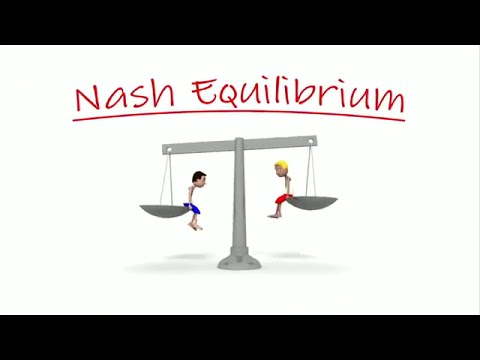
\includegraphics[]{equi.jpg}\\
    \caption{Nash}\\
    Source: https://i.ytimg.com/
    \label{game:3}
\end{figure}

Nash showed that there is a Nash equilibrium for every finite game
Game theorists use the Nash equilibrium concept to analyze the outcome of the strategic interaction of several decision makers. In other words, it provides a way of predicting what will happen if several people or several institutions are making decisions at the same time, and if the outcome for each of them depends on the decisions of the others. The simple insight underlying John Nash's idea is that one cannot predict the result of the choices of multiple decision makers if one analyzes those decisions in isolation. Instead, one must ask what each player would do, taking into account the decision-making of the others.
\newpage
\section{Nash Equilibrium for Prisoner's dilemma}
In a game where pure strategy is used Nash Equilibrium may or may not exist. 
 In the game of 
 \ref{tab:table1}
 prisoner's dilemma
 there is only one Nash Equilibirum, (Confess,Confess), i.e. both players will confess.

This can be proved as follows. When, P1 confesses, P2 is better off confessing than denying because he gets 5 years confessing which is less than 10 years

if he denies. When, P2 confesses, P1 is better off confessing than denying, because  P1 gets 5 years when he confesses but he gets 10 years on denying. The above analysis, shows that (C,C) represents Nash Equilibrium. Similarly, one can show that this is the only Nash Equilibrium in this game.
By examining the four possible pairs of actions in this game, one can see that the action pair (Confess,Confess) is a pure strategy Nash Equilibrium because if player 2 chooses Confess,player 1 is better off choosing Confess than Deny. Similarly given that player 1 chooses to Confess, player 2 is better off choosing Confess than Deny.
\newpage
\chapter{MiniMax Algorithm}
Minimax is a kind of
\href{https://en.wikipedia.org/wiki/Backtracking}{backtracking}
algorithm that is used in decision making and game theory to find the optimal move for a player, assuming that your opponent also plays optimally. It is widely used in two player turn-based games such as Tic-Tac-Toe, Backgammon, Mancala, Chess, etc.

In Minimax the two players are called maximizer and minimizer. The maximizer tries to get the highest score possible while the minimizer tries to do the opposite and get the lowest score possible.

Every board state has a value associated with it. In a given state if the maximizer has upper hand then, the score of the board will tend to be some positive value. If the minimizer has the upper hand in that board state then it will tend to be some negative value. The values of the board are calculated by some heuristics which are unique for every type of game.
\newpage
\textbf{Example: }
Consider a game which has 4 final states and paths to reach final state are from root to 4 leaves of a perfect binary tree as shown below. Assume you are the maximizing player and you get the first chance to move, i.e., you are at the root and your opponent at next level.\textbf{Which move you would make as a maximizing player considering that your opponent also plays optimally?}
\begin{figure}
    \centering
    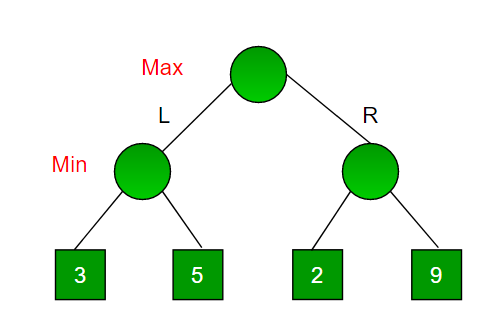
\includegraphics[]{minmax.png}
    \caption{minmax1}\\
    Source: geeksforgeeks.com/minmax
    \label{game4}
\end{figure}
Since this is a backtracking based algorithm, it tries all possible moves, then backtracks and makes a decision.
\begin{enumerate}
    \item Maximizer goes LEFT: It is now the minimizers turn. The minimizer now has a choice between 3 and 5. Being the minimizer it will definitely choose the least among both, that is 3
    \item Maximizer goes RIGHT: It is now the minimizers turn. The minimizer now has a choice between 2 and 9. He will choose 2 as it is the least among the two values.
\end{enumerate}
Being the maximizer you would choose the larger value that is 3. Hence the optimal move for the maximizer is to go LEFT and the optimal value is 3.
Now the game tree looks like below:
\begin{figure}
    \centering
    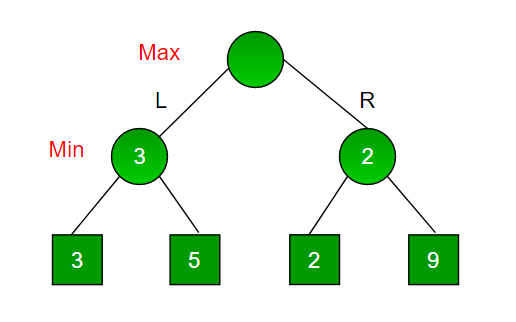
\includegraphics[]{minmax1.png}
    \caption{minmax2}\\
    Source: geeksforgeeks.com/minmax
    \label{game5}
\end{figure}
The above tree shows two possible scores when maximizer makes left and right moves.

Note: Even though there is a value of 9 on the right subtree, the minimizer will never pick that. We must always assume that our opponent plays optimally.

\newpage
\section{MiniMax Code}
Implementation of MiniMax algorithm in Java: 

\begin{lstlisting}
// A simple java program to find maximum score that 
// maximizing player can get. 
  
import java.io.*; 
  
class MinMax { 
    
  
// Returns the optimal value a maximizer can obtain. 
// depth is current depth in game tree. 
// nodeIndex is index of current node in scores[]. 
// isMax is true if current move is of maximizer, else false 
// scores[] stores leaves of Game tree. 
// h is maximum height of Game tree 
 static int minimax(int depth, int nodeIndex, boolean  isMax, 
            int scores[], int h) 
{ 
    // Terminating condition. i.e leaf node is reached 
    if (depth == h) 
        return scores[nodeIndex]; 
  
    // If current move is maximizer, find the maximum attainable 
    // value 
    if (isMax) 
    return Math.max(minimax(depth+1, nodeIndex*2, false, scores, h), 
            minimax(depth+1, nodeIndex*2 + 1, false, scores, h)); 
  
    // Else (If current move is Minimizer), find the minimum 
    // attainable value 
    else
        return Math.min(minimax(depth+1, nodeIndex*2, true, scores, h), 
            minimax(depth+1, nodeIndex*2 + 1, true, scores, h)); 
} 
  
// A utility function to find Log n in base 2 
 static int log2(int n) 
{ 
return (n==1)? 0 : 1 + log2(n/2); 
} 
  
// Driver code 
  
    public static void main (String[] args) { 
            // The number of elements in scores must be 
    // a power of 2. 
    int scores[] = {3, 5, 2, 9, 12, 5, 23, 23}; 
    int n = scores.length; 
    int h = log2(n); 
    int res = minimax(0, 0, true, scores, h); 
    System.out.println( "The optimal value is : "  +res);  
          
    } 
} 
\end{lstlisting}
\chapter{History}
Game theoretical concepts have been utilized to analyze problems for millennia, long
before game theory was a formally-defined field. One interesting example is that the Talmud, the Jewish holy book that provides the basis for Jewish law, prescribes solutions
for allocation of disputed resources that confounded scholars until the 1980s when mathematicians Robert Aumann and Michael Maschler solved the problem using the tools of
modern game theory. As it turns out, the solution given by the Talmud is to split the
disputed amount equally. Another example is when James Madison considered the effects of different taxation systems with game theoretical concepts. The list goes on, as
conflict resolution and strategic decision-making have been important issues throughout
all of human history.
The first work that brought about game theory as a formal field of mathematics
was Hungarian mathematician John von Neumann’s paper The Theory of Games in 1928. This paper had three major results. The first was reducing a game to the cases where
each player knows either everything or nothing about the other player’s previous moves.
He also proved the minimax theorem for two person zero-sum games, and he analyzed
three person zero-sum games.
Economist Oskar Morgenstern connected with von Neumann in 1938, and the
two then worked together on Theory of Games and Economic Behavior, published in
1944. This work was huge in the development of game theory. They expanded on von
Neumann’s previous work with an in-depth analysis of situations where players have only
partial knowledge of other players’ previous decisions, whereas The Theory of Games made
the assumption that players knew either everything or nothing about previous decisions.
They also expanded the definition of payoffs; previously payoffs were generally considered
to be only monetary, but von Neumann and Morgenstern developed the theory of utility,
which is still used today in many fields such as economics.
Since von Neumann and Morgenstern laid the foundation for game theory, it has
15
been added to by many mathematicians, such as John Nash in the 1950s. However, the
main development over the following decades was increasingly widespread application to
many fields. While certainly important in the field of economics, the use of game theory
has expanded to extensive use in biology, and it is also very important to the development
of military strategy. Interestingly, the five game theorists who have won the Nobel Prize
for economics also worked as advisors to the Pentagon over the courses of their careers. Game theory has also been applied in fields such as computer science and moral
philosophy.
\newpage
\chapter{Applications of Game Theory in CS}
\textbf{\large Cloud Computing}

In cloud computing, game theory is used for modeling complex interactions between cloud providers--whose aim is to minimize cost while maximizing resource utilization--on one hand and  a number of service providers often with conflicting objectives of maximizing Quality of Service at minimal cost. In such a situation, a game is set up based on an utility function that will eventually steer game play towards an equilibrium state, the Nash Equilibrium, where no players could receive an incentive to change their strategy--that state where objectives of all players are balanced. There are many scenarios in cloud resource management involving spot pricing of cloud resource addressed by auction/bidding games. \\
\textbf{\large Network Security}
A similar case applies in network security. Recently researchers have been developing both deterministic and stochastic security games to study security problems  as an optimization decision problem comprising multiple players notably the attackers and  the  defenders. \\
\textbf{\large Resource Allocation and Networking}
Computer network bandwidth can be viewed as a limited resource. The users on the network compete for that resource. Their competition can be simulated using game theory models. No centralized regulation of network usage is possible because of the diverse ownership of network resources.
The problem is of ensuring the fair sharing of network resources. For example, ten Stanford students on the same local network need access to the Internet. Each person, by using their network connection, diminishes the quality of the connection for the other users. This particular case is that of a volunteer's dilemma. That is, if one person abstains from using the network, the other people will be better off, but that person will be worse off.

If a centralized system could be developed which would govern the use of the shared resources, each person would get an assigned network usage time or bandwidth, thereby limiting each person's usage of network resources to his or her fair share.

As of yet, however, such a system remains an impossibility, making the situation of sharing network resources a competitive game between the users of the network and decreasing everyone's utility. \\
\textbf{\large Artificial Intelligence: }
One of the marks that differentiates a human from a machine is the human's ability to make independent decisions based on environmental stimuli. Most computer programs that are required to make any sort of a decision are currently pre-programmed with the lists of decisions based on a number of conditions. However, if those conditions are not met in some way or are altered, computers have no way of making decisions they were not programmed to make.
In the future, AI programs may be endowed with the ability to make new decisions unplanned for by their creators. This would require the programs to be able to generate new payoff matrices based on the observed stimuli and experience. A program that is able to do that would be capable of learning and would, in a lot of ways, resemble the human decision-making process.
\newpage
\bibliography{}
\typebf{References}
\begin{verbatim}
[1] CS_IITD (2002).
http://www.cse.iitd.ernet.in/~rahul/cs905/lecture1.html
[2] https://en.wikipedia.org/wiki/Game_theory
[3]https://sophia.stkate.edu/cgi/viewcontent.cgi?article=
1078&context=undergraduate_research_symposium
[4] MinMax theory Introduction
https://www.geeksforgeeks.org/minimax-algorithm-in
-game-theory-
set-1-introduction/
[5] http://www.cse.iitd.ernet.in/~rahul/cs905/
[6] Applications
https://cstheory.stackexchange.com/questions/16187
/applications-of-game-theory-in-computer-science
[7] P. Flynn (2005). A beginner’s introduction 
\end{verbatim}
\end{document}